\begin{exercice}\label{exoDS2012-1-0001}

La figure \ref{graphesin} r\'epresente le graphe de la fonction $f(x)=\sin(x)$, pour $x\in[-\pi,\pi]$. 

\begin{enumerate}
%\item Exprimez les fonctions suivantes sous la forme de fonctions compos\'ees associ\'ees \`a  $f$.
\item Est-ce que la fonction $f_1(x)=\sin(x^2)$ est paire ? Impaire ? P\'eriodique ? Si elle est p\'eriodique trouver sa p\'eriode. Justifier au mieux vos réponses.  
\item Esquisser le graphe des fonctions suivantes  
\end{enumerate}

 
\begin{multicols}{3}
  \begin{itemize}
    \renewcommand{\labelitemi}{$\bullet$}
  \item $f_1(x)=\sin(2x)$ ;
  \item $f_2(x)=2\sin(x)$ ;
  \item $f_3(x)=\sin^2(x)$ ;
  %\item $f_4(x)=\sin(x^2)$ ;
  \item $f_4(x)=\sin(x-1)$ ;
  \item $f_5(x)=\sin(x)-1$.
  \end{itemize}
\end{multicols}

\begin{figure}
 \begin{center}
  \caption{Le graphe de la fonction sinus}
   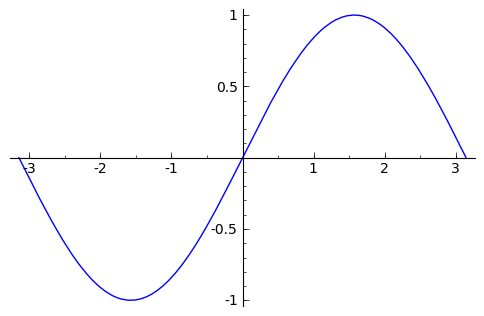
\includegraphics[width=6cm]{sin.png}\label{graphesin}
\end{center}
\end{figure}


\corrref{DS2012-1-0001}
\end{exercice}
